\documentclass{article}
\usepackage[utf8]{inputenc}

\title{Critical Computer Science Reading List}
\author{\textbf{Audrey Beard} \\
        beardj2@rpi.edu \\
        Computer Science Department \\
        Rensselaer Polytechnic Institute}
\date{\today}

\usepackage{natbib}
\usepackage{graphicx}

\begin{document}

\maketitle

\section{Introduction}
The intent of this document is to provide context for Critical Computer Science Pedagogy at Rensselaer Polytechnic Institute.
Being rooted in computer vision and machine learning, I undoubtedly bias my literature review towards those topics.
This document is broken into several sections, ranging from "pure" pedagogical theory, to science and technology studies (STS) literature, to "pure" computer science papers.

\section{Critical Computer Science Research}
\subsection{}

\begin{figure}[h!]
\centering
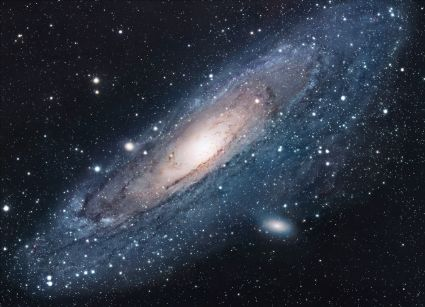
\includegraphics[scale=1.7]{universe}
\caption{The Universe}
\label{fig:universe}
\end{figure}

\section{Conclusion}
``I always thought something was fundamentally wrong with the universe'' \citep{adams1995hitchhiker}

\bibliographystyle{plain}
\bibliography{refs}
\end{document}
